The microscopic movies of growing bacteria by Trude et al.~\cite{Trude1982} contain various scenes
covering cases between only a few individual bacteria and large collections.
For our purpose, we extracted individual frames as images.
Afterwards, we used the omnipose~\cite{Cutler2022} segmentation tool to obtain cell masks of the
images. Since we chose an in-image color-based encoding scheme, it is of utmost importance that
color values for the same cell match between individual time points.
The total size of the domain and the duration of the movie were estimated using the provided citation
information and contextual clues, such as size of the bacteria themselves which was then compared to
literature values~\cite{Nelson2000}.

The bacterial diameters were estimated with $\approx\SI{0.5}{\micro\metre}$ and the time
interval spanning $8$ frames was estimated as $\SI{20}{\minute}$.
This results in a conversion value of $h=\SI{30}{\pixel\per\micro\metre}$.
Their particular numerical values are not relevant to the methods proposed in this work.
For studies targeting to extract precise numerical
values a closer inspection and clarification would be required.
The same parameter estimations can also be achieved by using pixel-based units.
Such changes will leave the profiles unchanged since both the units of the vertices $\vec{x}_i$ and
of the displacement uncertainty $\sigma$ will be rescaled which will cancel out.
This can be seen directly when inspecting equations~\ref{eq:parameter-estimation-log-likelihood} and
\ref{eq:parameter-estimation-least-squares}.
Furthermore, values of the Lineage-aware Image-Space metric
(equation~\ref{eq:Lineage-aware-image-space-metric}) will also be left untouched since the image
resolution does not change.

The obtained constants are listed in Table~\ref{tab:supplement-application-1-constants}.
As we have explained in the main text, the time series is split into an interval $T_1$ containing no
division events and an interval $T_2$ which includes a single division event.
We provide scripts that can be used to replicate our method of obtaining this dataset.
These can be found in the \texttt{data} folder of the GitHub repository:
\url{https://github.com/jonaspleyer/cr_mech_coli/}.

\begin{table}[H]
    \begin{tabularx}{\textwidth}{l r@{} @{\hspace{0.3em}}l X}
        \textbf{Constant} & \multicolumn{2}{l}{\textbf{Value}} & \textbf{Description}\\
        \toprule
        $T_\text{1}$ & $17.5$&$\unit{\minute}$ & Total time without division.\\
        $T_\text{2}$ & $74.375$&$\unit{\minute}$ & Total time including division events.\\
        & $998-1295$ && Range of frames extracted from movie.\\
        $h$ & $30$&$\unit{\pixel\per\micro\metre}$ & Conversion factor between pixels and lengths\\
        $N_\text{vertices}$ & $8$ && Number of vertices use for the discretized rod\\
        $\Delta x$ & $0.15$&$\unit{\micro\metre}$ & Displacement uncertainty used to calculate the
        profile-likelihood\\
        $L_x$ & $25.6$ & $\unit{\micro\metre}$ & Horizontal domain size.\\
            & $768$ & $\unit{\pixel}$\\
        $L_y$ & $19.2$ & $\unit{\micro\metre}$ & Vertical domain size.\\
            & $576$ & $\unit{\pixel}$\\
        \bottomrule
    \end{tabularx}
    \caption{Manually estimated constants which are used within the numerical simulation.}
    \label{tab:supplement-application-1-constants}
\end{table}
% \begin{enumerate}
%     \item Have masks of data; reference image segmantation tools; or do it by hand
%     \item ensure that colors are matching for bacteria between time-steps
%     \item clean borders of images if needed
%     \item know domain size; otherwise use pixels
% \end{enumerate}

Figure~\ref{fig:supplement-optimization-progression} shows the progression of the raw cost function
(not normalized by the squared uncertainty of the displacements) of the various optimizations.


\begin{figure}[H]
    \centering
    \begin{tikzonimage}[width=0.5\textwidth]
        {figures/crm_fit/optimization-progression.pdf}
        \node at (0, 1.1)[anchor=north west, black]{\textbf{A}};
    \end{tikzonimage}%
    \begin{tikzonimage}[width=0.5\textwidth]
        {figures/crm_divide/optimization-progression.pdf}
        \node at (0, 1.1)[anchor=north west, black]{\textbf{B}};
    \end{tikzonimage}%
    \caption{
        Optimization progression of the distinct model choices analyzed in Section~\ref{section:application-2}.
        All cost functions exhibit rapic decay before a final optimum is reached.
        The relative tolerance of the optimization algorithm was chosen conservatively low such that
        stability of the final optimum is ensured.
        (A) Progressions of cost functions for model choices without division events in units
        $[L]=\unit{\micro\metre\squared}$.
        (B) Cost function progression for the reduced Morse model with division events in units
        $[L]=\unit{\pixel\squared}$.
    }
    \label{fig:supplement-optimization-progression}
\end{figure}

Figure~\ref{fig:supplement-profiles-with-division} shows the missing profiles of growth rates of the
daughter cells left out in Figure~\ref{fig:likelihood-profiles-comparison-with-division}.
Some of these parameter values such as (A),(C) and (E) could be compatible with a vanishing growth
rate.
However these statements can only be completely justified if we can provide a good estimate for the
displacement uncertainty $\sigma$ in pixel space with respect to the  newly defined Lineage-aware
Image-Space metric.
This requires further mathematical attention to its definition.
Furthermore, results from section~\ref{section:application-2} have shown that growth rates and
division lengths can be estimated much more accurately when a division event is involved, thus
providing effectively a lower and upper bound on both values.
Furthermore, the results from Section~\ref{section:application-2} show that growth rates and
division lengths can be estimated much more accurately when a division event is involved.
This effectively provides a lower and upper bound on both values.
Small growth rates can result from insufficient data points being included after the initial
division event, such that the overall length of the bacteria appears constant in the short time
interval after division.

\begin{figure}[H]
    \begin{tikzonimage}[width=0.25\textwidth]
        {figures/crm_divide/profiles-pretty/pdf/profile-growth-rate-1-1.pdf}%
        \node at (0, 1.1)[anchor=north west, black]{\textbf{A}};
    \end{tikzonimage}%
    \begin{tikzonimage}[width=0.25\textwidth]
        {figures/crm_divide/profiles-pretty/pdf/profile-growth-rate-2-0.pdf}%
        \node at (0, 1.1)[anchor=north west, black]{\textbf{B}};
    \end{tikzonimage}%
    \begin{tikzonimage}[width=0.25\textwidth]
        {figures/crm_divide/profiles-pretty/pdf/profile-growth-rate-2-1.pdf}%
        \node at (0, 1.1)[anchor=north west, black]{\textbf{C}};
    \end{tikzonimage}%
    \begin{tikzonimage}[width=0.25\textwidth]
        {figures/crm_divide/profiles-pretty/pdf/profile-growth-rate-3-0.pdf}%
        \node at (0, 1.1)[anchor=north west, black]{\textbf{D}};
    \end{tikzonimage}\\
    \begin{tikzonimage}[width=0.25\textwidth]
        {figures/crm_divide/profiles-pretty/pdf/profile-growth-rate-3-1.pdf}%
        \node at (0, 1.1)[anchor=north west, black]{\textbf{E}};
    \end{tikzonimage}%
    \begin{tikzonimage}[width=0.25\textwidth]
        {figures/crm_divide/growth-rate-distribution.pdf}%
        \node at (0, 1.1)[anchor=north west, black]{\textbf{F}};
    \end{tikzonimage}%
    \caption{
        (A-E) Remaining parameter profiles for the growth rates of the daughter cells.
        This extends Figure~\ref{fig:likelihood-profiles-comparison-with-division}.
        The profile show that the parameters can be informed by the provided data.
        (F) Distribution of estimated growth rates distinguishing between mother (dark blue) and
        daughter (light blue) cells.
    }
    \label{fig:supplement-profiles-with-division}
\end{figure}

In order to assess the accuracy of the estimated parameters in relation to our model, we can examine
the contributions to the cost function at each time point in the simulation.
We expect that the differences indicated by the cost function are minimal at the start point and
grow as time progresses.
Our system ins inherently non-linear, containing exponential growth and complex interaction forces.
This means that any parameter choice which is not optimal can lead to large deviations with
increasing time.
For a Lipschitz-continous system, this deviation can be bound by an exponential envelope of
differences surrounding the true values, which results in an exponential temporal progression of the
cost function itself.

Figure~\ref{fig:supplement-cost-evolution-time} shows the contributions of the individual time
points to the total Lineage-aware Image-Space metric.
As expected, the fully optimized system (orange) does not contain any cases where the parent penalty
$p_p$ is utilized.
When increasing the growth rates of all cells by $20\%$ (blue curves), we can see the non-linear
nature of our system come into play.
This change leads to a division time much earlier than in the fully optimized case which therefore
makes use of the parent penalty $p_p$.
The blue curves show 3 scenarios assigning $p_p=1,0.5,0$ respectively.
These values show a smooth transition between fully accounting for parental differences $p_p=1$ to
not accounting for them at all $p_p=0$.

The presented curves exhibit two distinct exponential slopes which are separated by the division
event.
This can be observed most accurately in the fully optimized system (orange) where the vertical gray
line indicates the start of the secondary exponential.
Such a clear distinction between initial growth phase of the mother cells and secondary growth phase
of the daughter cells is only possible in this particular scenario where the division events of the
bacteria are within close temporal proximity to each other.

\begin{figure}[H]
    \centering
    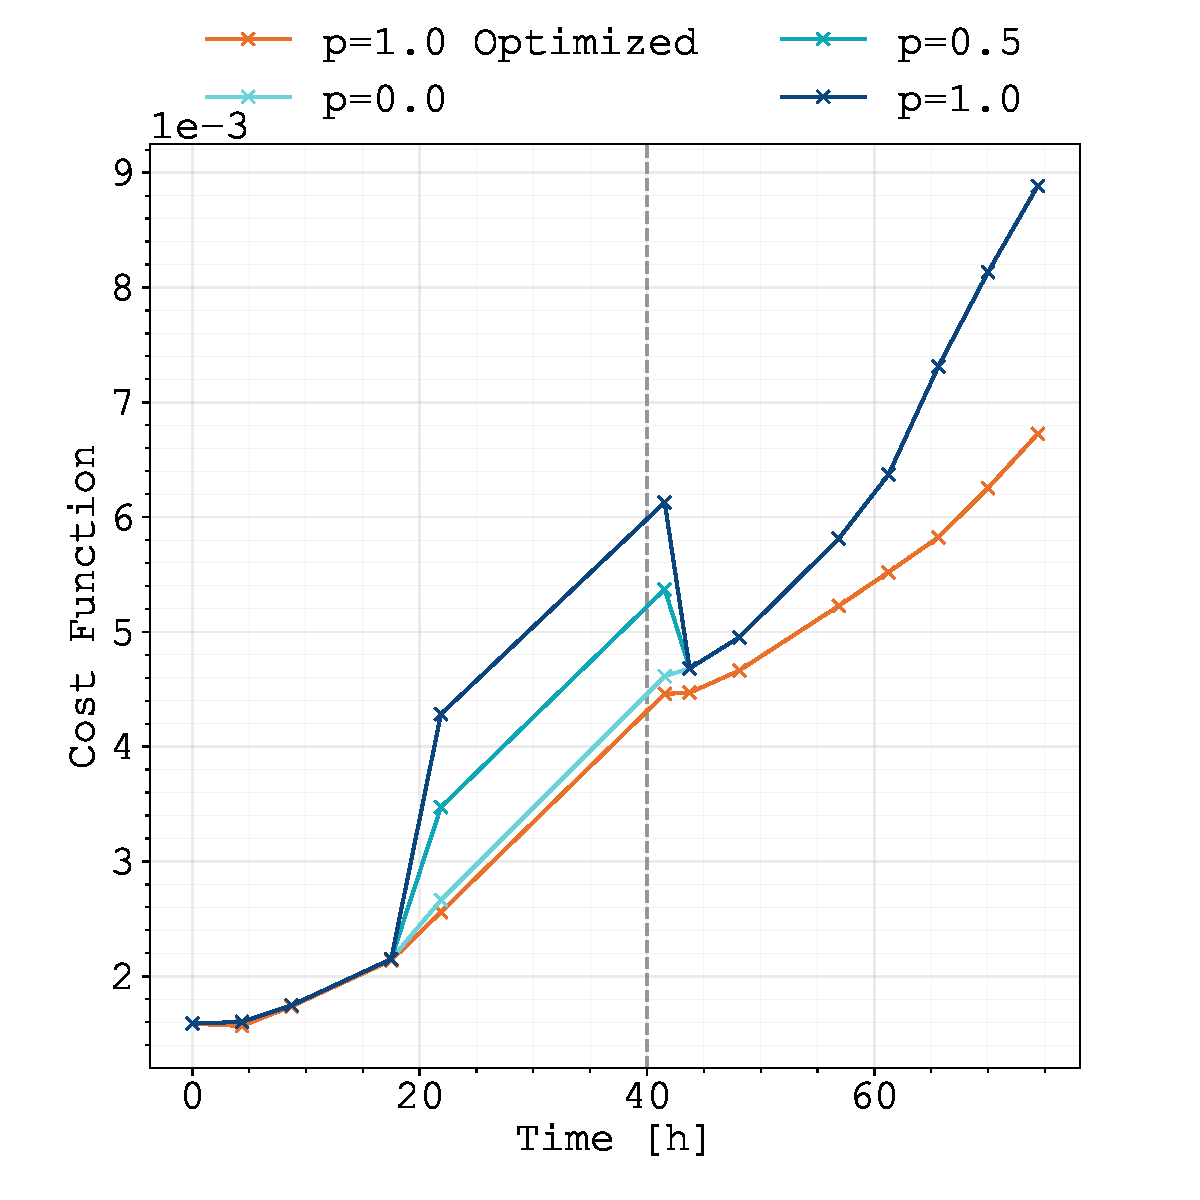
\includegraphics[width=0.5\textwidth]{figures/crm_divide/time-evolution.pdf}%
    \caption{
        Contributions to the Lineage-aware Image-Space metric at evaluated time points of the
        simulation.
        The fully optimized system (orange) does not contain any configurations in which a parent
        penalty $p_p$ is utilized.
        When increasing the growth rates of each cell by $20\%$, we can clearly see the effect of
        the parent penalty.
        The case $p_p=1$ will result in full weighting of parental differences, while $p_p=0.5$
        assigns only partial weighting and $p_p=0$ ignores them.
    }
    \label{fig:supplement-cost-evolution-time}
\end{figure}

%###################################################################################################
% \subsection{More Simulation Aspects (TODO)}
% \label{section:supplement-more-simulation-aspects}
% %TODO insert this into the discussion later
% \begin{table}[H]
%     \centering
%     \def\arraystretch{1.3}
%     \begin{tabularx}{\textwidth}{c l X}
%         &\textbf{Aspect} & \textbf{Description}\\
%         \toprule
%         &\textbf{(C) Cellular}\\
%         \midrule
%         (1) & Rod-Shaped Mechanics &
%             Rod-shaped bacteria are flexible rods which are able to freely move around (off-lattice
%             approach) \cite{Takeuchi2005,Ursell2014,Amir2014_2}.\\
%         (2) & Growth &
%             Cells grow exponentially by inserting new material either along the circular part of the
%             rod or at the tip~\cite{Robert2014,Takeuchi2005}.\\
%         (3) & Differentiation &
%             \ac{bsubtilis} is known to differentiate into matrix-producing and
%             surfactin-producing cells \cite{vanGestel2015,Lpez2010}.\\
%         (4) & Division &
%             The formation and continuation of van Gogh bundles is driven by cell division
%             \cite{vanGestel2015}.
%             Bacteria can form multilayers during their growth phase \cite{Duvernoy2018}.\\
%         (5) & Variable Parameters &
%             Parameters for individual cells are not fixed values but rather taken from a
%             distribution \cite{Koutsoumanis2013}.\\
%         &\textbf{(CC) Cell-Cell Interactions}\\
%         \midrule
%         (6) & Adhesion &
%             Bacteria adhere to each other at longer distances and attach when in close contact
%             \cite{Verwey1947,Trejo2013}.
%             The interaction between rods can be polarized \cite{Duvernoy2018}.\\
%         (7) & Friction &
%             Friction between cells \cite{Grant2014} can be asymmetrical \cite{Doumic2020}.\\
%         &\textbf{(DC) Domain-Cell Interactions}\\
%         \midrule
%         (8) & External Forces &
%             Bacteria tend to stick to surfaces \cite{vanLoosdrecht1989}.
%             The extracellular gel exerts a force onto the cells \cite{Grant2014}.\\
%         (9) & Extracellular Reactions &
%             Bacteria can take up nutrients or possible secrete/take up signalling molecules
%             \cite{Li2025}.\\
%         \bottomrule
%     \end{tabularx}
%     \label{table:simulation-aspects-supplement}
%     \caption{
%         This table extends table~\ref{table:simulation-aspects} with additional observations.
%         It has to be noted that this table includes more specific behavior that might not be
%         generalizable across all types of rod-shaped bacteria.
%     }
% \end{table}
% 
% \begin{itemize}
%     \item new class of aspects: (DC) Domain-Cell Interactions
%     \item List which aspects are here additionally
%     \item discuss which of them might need specific models and can not be paired with others
%     \item which can be bundled together without problems?
% \end{itemize}

%###################################################################################################
% \paragraph*{Implementation \& Performance (TODO)}
% \label{section:supplement-performance}
%
% On the programming side, we are using the \texttt{pyo3} and \texttt{maturin} crates which allow us
% to easily generate Python bindings and enable us to interoperate between the two ecosystems.
%
% By using \texttt{cellular\_raza}, we can make use of multiple threads for running a single numerical
% simulation, using the built-in parallelization methods (see Supplementary Material,
% Figure~\ref{fig:timings-crm_divide}).
%
% \begin{itemize}
%     \item Quadratic Scaling (see figure~\ref{fig:timings-crm_divide}) comes from more dense
%         simulation
%     \item Overall number of agents which can be simulated is satisfactory for current purposes
%     \item Improvement from $1 \Rightarrow 2$ and $2\Rightarrow4$ threads; first is major; second
%         only minor
%     \item Flamegraph still shows much cycles running against hurdles::Barrier::wait $\Rightarrow$
%         this leaves room for improvement
%     \item Flamegraph also shows that $\approx 75\%$ of all cycles is related to actual work (not
%         just waiting).
%         In particular to update\_mechanics functions.
% \end{itemize}
%
% \begin{figure}[H]
%     \centering
%     \begin{tikzonimage}[width=0.5\textwidth]
%         {figures/docs/computation-time-with-initial-agents.pdf}
%         \node at (0, 1)[anchor=north west]{\textbf{A}};
%     \end{tikzonimage}%
%     \begin{tikzonimage}[width=0.5\textwidth]
%         {figures/crm_divide/timings.pdf}
%         \node at (0, 1)[anchor=north west]{\textbf{B}};
%     \end{tikzonimage}\\
%     \begin{tikzonimage}[width=\textwidth]
%         {figures/docs/flamegraph.pdf}
%         \node at (0.02, 0.98)[anchor=north west]{\textbf{C}};
%     \end{tikzonimage}\\
%     \caption{
%         (A) Wall time of the performed simulation with increasing number of final agents inside the
%         simulation domain.
%         (B) Distribution of computation time for the division script utilized in
%         section~\ref{sec:application-1-with-division}.
%         (C) Flamegraph of a typical simulation showcasing frequency of function calls for
%         parallelized execution of simulations.
%     }
%     \label{fig:timings-crm_divide}
% \end{figure}
